\chapter{Primitives et Intégration}

Ce chapitre présente le calcul intégral, l'une des branches les plus fécondes de l'analyse. Nous allons définir les primitives d'une fonction, puis l'intégrale comme outil de calcul d'aires, de moyennes et de modélisation mathématique.

\section{Primitives d'une Fonction}

\subsection{Définition et propriétés}

Rechercher les primitives d'une fonction est l'opération inverse de la dérivation.

\begin{definition}[Primitive]
Soit $f$ une fonction définie sur un intervalle $I$.
On appelle **primitive** de $f$ sur $I$ toute fonction $F$ dérivable sur $I$ telle que pour tout $x \in I$ :
\[
F'(x) = f(x)
\]
\end{definition}

\begin{theoreme}[Existence et ensemble des primitives]
\begin{itemize}
    \item Toute fonction **continue** sur un intervalle $I$ admet des primitives sur $I$.
    \item Si $F$ est une primitive de $f$ sur $I$, alors toute autre primitive $G$ de $f$ sur $I$ est de la forme :
    \[
    G(x) = F(x) + C
    \]
    où $C$ est une constante réelle.
\end{itemize}
\end{theoreme}

\subsection{Primitives des fonctions usuelles}

Le tableau suivant rassemble les formules de primitives obtenues par lecture inverse du tableau des dérivées :

\begin{table}[h!]
\centering
\begin{tabular}{|c|c|c|}
\hline
\textbf{Fonction} $f(x)$ & \textbf{Une primitive} $F(x)$ & \textbf{Intervalle} $I$ \\
\hline
$k$ (constante) & $kx$ & $\R$ \\
$x^n$ ($n \in \N$) & $\frac{x^{n+1}}{n+1}$ & $\R$ \\
$\frac{1}{x^2}$ & $-\frac{1}{x}$ & $]-\infty, 0[$ ou $]0, +\infty[$ \\
$\frac{1}{\sqrt{x}}$ & $2\sqrt{x}$ & $]0, +\infty[$ \\
$e^x$ & $e^x$ & $\R$ \\
$\frac{1}{x}$ & $\ln(x)$ & $]0, +\infty[$ \\
\hline
\end{tabular}
\caption{Primitives des fonctions usuelles}
\end{table}

\subsection{Primitives et composition}

Pour trouver des primitives de fonctions plus complexes, on repère des formes de dérivées de fonctions composées :

\begin{table}[h!]
\centering
\begin{tabular}{|c|c|c|}
\hline
\textbf{Forme de la fonction} & \textbf{Une primitive} & \textbf{Condition sur} $u$ \\
\hline
$u' u^n$ ($n \in \N^*$) & $\frac{u^{n+1}}{n+1}$ & dérivable \\
$\frac{u'}{u^2}$ & $-\frac{1}{u}$ & $u(x) \ne 0$ \\
$\frac{u'}{\sqrt{u}}$ & $2\sqrt{u}$ & $u(x) > 0$ \\
$u' e^u$ & $e^u$ & dérivable \\
$\frac{u'}{u}$ & $\ln(u)$ & $u(x) > 0$ \\
\hline
\end{tabular}
\caption{Primitives de fonctions composées}
\end{table}

\section{Le Calcul Intégral}

\subsection{Définition de l'intégrale}

\begin{definition}[Intégrale]
Soit $f$ une fonction continue sur $[a, b]$ et $F$ une primitive de $f$ sur $[a, b]$.
L'**intégrale** de $f$ de $a$ à $b$ est le nombre réel, noté $\int_a^b f(x) \dd x$, défini par :
\[
\int_a^b f(x) \dd x = [F(x)]_a^b = F(b) - F(a)
\]
\end{definition}

\subsection{Interprétation géométrique (Aire)}

Lorsque la fonction $f$ est continue et positive sur l'intervalle $[a, b]$, l'intégrale $\int_a^b f(x) \dd x$ est égale à l'aire $\mathcal{A}$ de la région délimitée par la courbe $\mathcal{C}_f$, l'axe des abscisses et les droites verticales d'équations $x=a$ et $x=b$ (exprimée en unités d'aire, u.a.).

\begin{center}
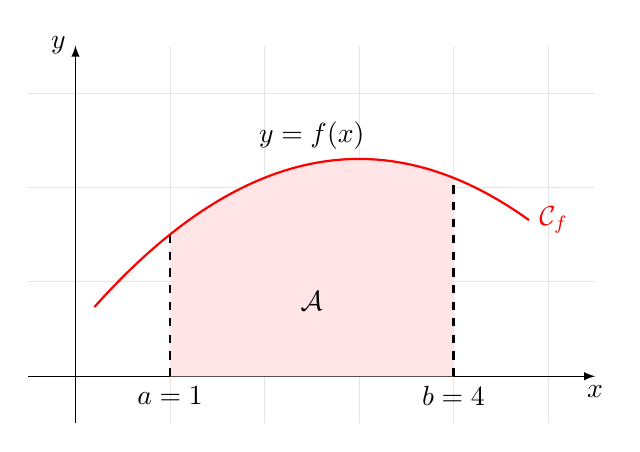
\begin{tikzpicture}[scale=1.2]
  % Grille
  \draw[gray!20,very thin] (-0.5,-0.5) grid (5.5,3.5);
  % Axes
  \draw[->,>=latex] (-0.5,0) -- (5.5,0) node[below] {$x$};
  \draw[->,>=latex] (0,-0.5) -- (0,3.5) node[left] {$y$};
  
  % Remplissage de l'aire sous la courbe
  \fill[red!10] (1,0) -- plot[domain=1:4] (\x, {-0.2*\x^2 + 1.2*\x + 0.5}) -- (4,0) -- cycle;
  
  % Courbe représentative
  \draw[domain=0.2:4.8, samples=100, color=red, thick] plot (\x, {-0.2*\x^2 + 1.2*\x + 0.5}) node[right] {$\mathcal{C}_f$};
  
  % Droites de limites
  \draw[dashed, thick] (1,0) node[below] {$a=1$} -- (1,1.5);
  \draw[dashed, thick] (4,0) node[below] {$b=4$} -- (4,2.1);
  
  % Label
  \node at (2.5, 0.8) {$\mathcal{A}$};
  \node[above] at (2.5, 2.3) {$y=f(x)$};
\end{tikzpicture}
\end{center}

\subsection{Propriétés de l'intégrale}

Pour toutes fonctions $f$ et $g$ continues sur $[a, b]$ et tous réels $\alpha, \beta$ :
\begin{itemize}
    \item \textbf{Linéarité} : $\int_a^b (\alpha f(x) + \beta g(x)) \dd x = \alpha \int_a^b f(x) \dd x + \beta \int_a^b g(x) \dd x$.
    \item \textbf{Relation de Chasles} : Pour tout $c \in [a, b]$, $\int_a^b f(x) \dd x = \int_a^c f(x) \dd x + \int_c^b f(x) \dd x$.
    \item \textbf{Positivité et Ordre} : Si $f(x) \ge 0$ sur $[a,b]$, alors $\int_a^b f(x) \dd x \ge 0$. Si $f(x) \le g(x)$, alors $\int_a^b f(x) \dd x \le \int_a^b g(x) \dd x$.
\end{itemize}

\subsection{Valeur moyenne d'une fonction}

\begin{definition}[Valeur moyenne]
Soit $f$ une fonction continue sur un intervalle $[a, b]$ (avec $a < b$).
La **valeur moyenne** $\mu$ de $f$ sur $[a, b]$ est le réel :
\[
\mu = \frac{1}{b-a} \int_a^b f(x) \dd x
\]
\end{definition}

\section{L'Intégration par Parties (IPP)}

Lorsque l'on cherche l'intégrale d'un produit de deux fonctions dont on ne repère pas de forme de composée immédiate, on utilise la méthode d'intégration par parties.

\begin{theoreme}[Intégration par parties]
Soient $u$ et $v$ deux fonctions dérivables sur $[a, b]$ dont les dérivées $u'$ and $v'$ sont continues sur $[a, b]$. On a :
\[
\int_a^b u'(x) v(x) \dd x = \Big[ u(x) v(x) \Big]_a^b - \int_a^b u(x) v'(x) \dd x
\]
\end{theoreme}

\section{Équations Différentielles}

Une équation différentielle est une équation dont l'inconnue est une fonction, et dans laquelle apparaissent une ou plusieurs dérivées de cette fonction.

\subsection{Équations différentielles du premier ordre : $y' = ay + b$}

\begin{theoreme}[Solutions de $y' = ay + b$]
Soit $a$ et $b$ deux réels.
\begin{itemize}
    \item Si $a = 0$, l'équation s'écrit $y' = b$. Les solutions sont les fonctions de la forme :
    \[
    y(x) = bx + C \quad (\text{où } C \in \R)
    \]
    \item Si $a \ne 0$, les solutions de l'équation $y' = ay + b$ sur $\R$ sont les fonctions de la forme :
    \[
    y(x) = C e^{ax} - \frac{b}{a} \quad (\text{où } C \in \R)
    \]
\end{itemize}
\end{theoreme}

\begin{propriete}[Solution unique vérifiant une condition initiale]
Pour tous réels $x_0$ et $y_0$, il existe une **unique** solution $f$ de l'équation $y' = ay + b$ vérifiant la condition initiale $f(x_0) = y_0$.
\end{propriete}

\subsection{Équations différentielles du second ordre : $y'' + ay' + by = 0$}

Considérons l'équation $y'' + ay' + by = 0$ où $a$ et $b$ sont des réels.
Pour la résoudre, on associe l'équation du second degré dans $\Cnum$ appelée **équation caractéristique** :
\[
r^2 + ar + b = 0
\]
Soit $\Delta = a^2 - 4b$ son discriminant.

\begin{theoreme}[Solutions de $y'' + ay' + by = 0$]
\begin{itemize}
    \item \textbf{Si $\Delta > 0$} : L'équation caractéristique admet deux racines réelles distinctes $r_1$ et $r_2$.
    Les solutions de l'équation différentielle sur $\R$ sont les fonctions de la forme :
    \[
    y(x) = \alpha e^{r_1 x} + \beta e^{r_2 x} \quad (\text{où } \alpha, \beta \in \R)
    \]
    \item \textbf{Si $\Delta = 0$} : L'équation caractéristique admet une unique racine réelle double $r_0$.
    Les solutions de l'équation différentielle sur $\R$ sont les fonctions de la forme :
    \[
    y(x) = (\alpha x + \beta) e^{r_0 x} \quad (\text{où } \alpha, \beta \in \R)
    \]
    \item \textbf{Si $\Delta < 0$} : L'équation caractéristique admet deux racines complexes conjuguées $p + \iud q$ et $p - \iud q$ (avec $q \ne 0$).
    Les solutions de l'équation différentielle sur $\R$ sont les fonctions de la forme :
    \[
    y(x) = e^{px} \Big( \alpha \cos(qx) + \beta \sin(qx) \Big) \quad (\text{où } \alpha, \beta \in \R)
    \]
\end{itemize}
\end{theoreme}

\section{Méthodes Clés}

\begin{methode}[Calculer une intégrale par IPP]
Pour appliquer l'intégration par parties pour calculer $\int_a^b f(x) \dd x$ :
\begin{enumerate}
    \item **Écrire la fonction** sous la forme d'un produit $u'(x)v(x)$.
    \item **Choisir judicieusement** $u'(x)$ et $v(x)$ (en général, on dérive les polynômes ou logarithmes, et on intègre les exponentielles ou trigonométriques).
    \item **Calculer** $u(x)$ (une primitive de $u'$) et $v'(x)$ (la dérivée de $v$).
    \item **Appliquer** la formule de l'IPP et simplifier le résultat.
\end{enumerate}
\end{methode}

\begin{exemple}[Calcul par IPP]
Calculons l'intégrale : $I = \int_0^1 x e^x \dd x$.
Posons :
\[
\begin{cases}
v(x) = x & \implies v'(x) = 1 \\
u'(x) = e^x & \implies u(x) = e^x
\end{cases}
\]
Les fonctions $u$ et $v$ sont bien dérivables, et leurs dérivées sont continues sur $[0,1]$.
Par intégration par parties :
\[
I = \Big[ x e^x \Big]_0^1 - \int_0^1 1 \times e^x \dd x = (1 \cdot e^1 - 0 \cdot e^0) - \Big[ e^x \Big]_0^1 = e - (e^1 - e^0) = 1
\]
\end{exemple}

\section{Exercices d'Entraînement Résolus}

\subsection*{Exercice 1 : Primitive simple avec condition}
Déterminer la primitive $F$ de la fonction $f(x) = 3x^2 - x + 1$ sur $\R$ qui s'annule en 0.

\textbf{Solution :}
Les primitives de la fonction polynomiale $f$ sont de la forme :
\[
F(x) = 3\left(\frac{x^3}{3}\right) - \frac{x^2}{2} + x + C = x^3 - \frac{x^2}{2} + x + C
\]
où $C \in \R$.
On cherche la primitive qui s'annule en 0, soit :
\[
F(0) = 0 \iff 0^3 - \frac{0^2}{2} + 0 + C = 0 \iff C = 0
\]
La primitive cherchée est la fonction $F$ définie sur $\R$ par :
\[
F(x) = x^3 - \frac{x^2}{2} + x
\]

\subsection*{Exercice 2 : Primitive de la forme $u'/u$}
Déterminer une primitive de la fonction $f$ définie sur $]-1, +\infty[$ par :
\[
f(x) = \frac{3x^2}{x^3 + 1}
\]

\textbf{Solution :}
Posons $u(x) = x^3 + 1$. La fonction $u$ est strictement positive et dérivable sur $]-1, +\infty[$ avec $u'(x) = 3x^2$.
La fonction $f$ s'écrit donc sous la forme $\frac{u'}{u}$.
Une primitive de $f$ sur cet intervalle est :
\[
F(x) = \ln(u(x)) = \ln(x^3 + 1)
\]

\subsection*{Exercice 3 : Primitive de la forme $u' e^u$}
Déterminer une primitive de la fonction $f$ définie sur $\R$ par :
\[
f(x) = x e^{x^2 + 1}
\]

\textbf{Solution :}
Posons $u(x) = x^2 + 1$. La fonction $u$ est dérivable sur $\R$ avec $u'(x) = 2x$.
Exprimons $f(x)$ en fonction de $u'$ :
\[
f(x) = \frac{1}{2} (2x) e^{x^2 + 1} = \frac{1}{2} u'(x) e^{u(x)}
\]
La fonction $f$ est de la forme $\frac{1}{2} u' e^u$.
Une primitive de $f$ sur $\R$ est :
\[
F(x) = \frac{1}{2} e^{u(x)} = \frac{1}{2} e^{x^2 + 1}
\]

\subsection*{Exercice 4 : Primitive de la forme $u' u^n$}
Déterminer une primitive de la fonction $f$ définie sur $\R$ par :
\[
f(x) = (2x + 1)^4
\]

\textbf{Solution :}
Posons $u(x) = 2x + 1$. La fonction $u$ est dérivable sur $\R$ avec $u'(x) = 2$.
Exprimons $f(x)$ en fonction de $u'$ :
\[
f(x) = \frac{1}{2} \times 2 (2x + 1)^4 = \frac{1}{2} u'(x) (u(x))^4
\]
La fonction $f$ est de la forme $\frac{1}{2} u' u^4$.
Une primitive de $f$ sur $\R$ est :
\[
F(x) = \frac{1}{2} \times \frac{u^5}{5} = \frac{1}{10} (2x + 1)^5
\]

\subsection*{Exercice 5 : Primitive de la forme $u'/\sqrt{u}$}
Déterminer une primitive de la fonction $f$ définie sur $]-1/3, +\infty[$ par :
\[
f(x) = \frac{1}{\sqrt{3x + 1}}
\]

\textbf{Solution :}
Posons $u(x) = 3x + 1$. Sur $]-1/3, +\infty[$, $u(x) > 0$. Sa dérivée est $u'(x) = 3$.
Exprimons $f(x)$ en fonction de $u'$ :
\[
f(x) = \frac{1}{3} \times \frac{3}{\sqrt{3x+1}} = \frac{1}{3} \times \frac{u'(x)}{\sqrt{u(x)}} = \frac{2}{3} \times \frac{u'(x)}{2\sqrt{u(x)}}
\]
La fonction est de la forme $\frac{2}{3} \frac{u'}{2\sqrt{u}}$.
Une primitive de $f$ sur cet intervalle est :
\[
F(x) = \frac{2}{3} \sqrt{u(x)} = \frac{2}{3} \sqrt{3x + 1}
\]

\subsection*{Exercice 6 : Calcul d'intégrale simple}
Calculer l'intégrale suivante :
\[
I = \int_0^1 (3x^2 - 2x + 1) \dd x
\]

\textbf{Solution :}
Une primitive de la fonction $x \mapsto 3x^2 - 2x + 1$ est $F(x) = x^3 - x^2 + x$.
On a :
\[
I = \Big[ x^3 - x^2 + x \Big]_0^1 = (1^3 - 1^2 + 1) - (0^3 - 0^2 + 0) = 1 - 0 = 1
\]

\subsection*{Exercice 7 : Intégrale de la fonction inverse}
Calculer l'intégrale suivante :
\[
J = \int_1^e \frac{1}{x} \dd x
\]

\textbf{Solution :}
Une primitive de la fonction $x \mapsto \frac{1}{x}$ sur $]0, +\infty[$ est $F(x) = \ln(x)$.
On a :
\[
J = \Big[ \ln(x) \Big]_1^e = \ln(e) - \ln(1) = 1 - 0 = 1
\]

\subsection*{Exercice 8 : Intégrale de fonction trigonométrique}
Calculer l'intégrale suivante :
\[
K = \int_0^{\pi} \sin(x) \dd x
\]

\textbf{Solution :}
Une primitive de la fonction $x \mapsto \sin(x)$ est $F(x) = -\cos(x)$.
On a :
\[
K = \Big[ -\cos(x) \Big]_0^{\pi} = -\cos(\pi) - (-\cos(0)) = -(-1) + 1 = 1 + 1 = 2
\]

\subsection*{Exercice 9 : Calcul de la valeur moyenne}
Déterminer la valeur moyenne de la fonction $f(x) = 3x^2$ sur l'intervalle $[1, 3]$.

\textbf{Solution :}
La valeur moyenne est donnée par la formule :
\[
\mu = \frac{1}{3-1} \int_1^3 3x^2 \dd x = \frac{1}{2} \int_1^3 3x^2 \dd x
\]
Une primitive de $3x^2$ est $F(x) = x^3$.
\[
\int_1^3 3x^2 \dd x = \Big[ x^3 \Big]_1^3 = 3^3 - 1^3 = 27 - 1 = 26
\]
On obtient :
\[
\mu = \frac{1}{2} \times 26 = 13
\]

\subsection*{Exercice 10 : Autre forme $u'/u$ avec exponentielle}
Déterminer une primitive de la fonction $f$ définie sur $\R$ par :
\[
f(x) = \frac{e^x}{e^x + 2}
\]

\textbf{Solution :}
Posons $u(x) = e^x + 2$. La fonction $u$ est dérivable et strictement positive sur $\R$ avec $u'(x) = e^x$.
La fonction $f$ s'écrit sous la forme $\frac{u'}{u}$.
Une primitive de $f$ sur $\R$ est :
\[
F(x) = \ln(u(x)) = \ln(e^x + 2)
\]

\subsection*{Exercice 11 : Équation différentielle du premier ordre}
Résoudre sur $\R$ l'équation différentielle $y' - 3y = 6$ et déterminer l'unique solution $f$ telle que $f(0) = 1$.

\textbf{Solution :}
1. L'équation s'écrit $y' = 3y + 6$. C'est une équation de la forme $y' = ay + b$ avec $a=3 \ne 0$ et $b=6$.
   Les solutions générales sur $\R$ sont de la forme :
   \[
   y(x) = C e^{3x} - \frac{6}{3} = C e^{3x} - 2 \quad (\text{où } C \in \R)
   \]
2. Déterminons la solution $f$ vérifiant $f(0) = 1$ :
   \[
   f(0) = 1 \iff C e^{3(0)} - 2 = 1 \iff C - 2 = 1 \iff C = 3
   \]
La solution unique cherchée est la fonction $f$ définie sur $\R$ par :
\[
f(x) = 3 e^{3x} - 2
\]

\subsection*{Exercice 12 : Équation différentielle du second ordre}
Résoudre sur $\R$ l'équation différentielle suivante :
\[
y'' - 2y' + 2y = 0
\]

\textbf{Solution :}
C'est une équation différentielle linéaire homogène du second ordre à coefficients réels.
Écrivons son équation caractéristique associée :
\[
r^2 - 2r + 2 = 0
\]
Calculons son discriminant :
\[
\Delta = (-2)^2 - 4(1)(2) = 4 - 8 = -4
\]
Puisque $\Delta < 0$, l'équation caractéristique admet deux racines complexes conjuguées :
\[
r_1 = \frac{2 - \iud\sqrt{4}}{2} = 1 - \iud \quad \text{et} \quad r_2 = 1 + \iud
\]
Ici, la partie réelle est $p = 1$ et la partie imaginaire est $q = 1$.
D'après le théorème du cours, les solutions de l'équation différentielle sur $\R$ sont les fonctions de la forme :
\[
y(x) = e^x \Big( \alpha \cos(x) + \beta \sin(x) \Big) \quad (\text{où } \alpha, \beta \in \R)
\]

\section{Problèmes Résolus}

\subsection*{Problème 1 : Calcul d'aire délimitée par deux courbes}
On considère la fonction $f$ définie sur $[0, 1]$ par $f(x) = x^2$ et la fonction $g$ définie sur $[0, 1]$ par $g(x) = \sqrt{x}$. On note $\mathcal{C}_f$ et $\mathcal{C}_g$ leurs courbes représentatives.
\begin{enumerate}
    \item Démontrer que pour tout $x \in [0, 1]$, $g(x) \ge f(x)$.
    \item Calculer l'aire $\mathcal{A}$ de la région délimitée par les deux courbes $\mathcal{C}_f$ et $\mathcal{C}_g$ et les droites verticales d'équations $x=0$ et $x=1$ (exprimer le résultat en unités d'aire).
\end{enumerate}

\textbf{Solution :}
\begin{enumerate}
    \item Pour comparer $f(x)$ et $g(x)$ sur $[0, 1]$, calculons la différence :
    \[
    g(x) - f(x) = \sqrt{x} - x^2 = \sqrt{x}(1 - x\sqrt{x}) = \sqrt{x}(1 - x^{3/2})
    \]
    Pour tout $x \in [0, 1]$, on a $0 \le x \le 1 \implies 0 \le x^{3/2} \le 1 \implies 1 - x^{3/2} \ge 0$.
    Le produit est donc positif ou nul sur $[0, 1]$, ce qui montre que $g(x) \ge f(x)$.
    
    \item L'aire $\mathcal{A}$ de la région délimitée par les courbes est l'intégrale de la différence :
    \[
    \mathcal{A} = \int_0^1 (g(x) - f(x)) \dd x = \int_0^1 \left( \sqrt{x} - x^2 \right) \dd x
    \]
    Déterminons une primitive de $x \mapsto x^{1/2} - x^2$ :
    \[
    F(x) = \frac{x^{3/2}}{3/2} - \frac{x^3}{3} = \frac{2}{3}x\sqrt{x} - \frac{x^3}{3}
    \]
    Calculons l'intégrale :
    \[
    \mathcal{A} = \Big[ F(x) \Big]_0^1 = F(1) - F(0) = \left( \frac{2}{3}(1)(1) - \frac{1}{3} \right) - 0 = \frac{2}{3} - \frac{1}{3} = \frac{1}{3} \text{ u.a.}
    \]
    L'aire de la région en forme de fuseau fermée par les deux paraboles est égale à $1/3$ d'unité d'aire.
\end{enumerate}

\subsection*{Problème 2 : Étude d'une fonction définie par une intégrale}
Soit la fonction $F$ définie sur $\R$ par :
\[
F(x) = \int_0^x e^{-t^2} \dd t
\]
\begin{enumerate}
    \item Justifier que la fonction $F$ est dérivable sur $\R$ et donner sa dérivée $F'(x)$.
    \item En déduire le sens de variation de $F$ sur $\R$.
    \item Démontrer que pour tout $t \ge 1$, $t^2 \ge t$, puis en déduire que $e^{-t^2} \le e^{-t}$.
    \item Montrer que pour tout $x \ge 1$ :
    \[
    F(x) \le F(1) + \frac{1}{e} - e^{-x}
    \]
    En déduire que la fonction $F$ est majorée sur $[0, +\infty[$. Que peut-on en déduire pour sa limite en $+\infty$ ?
\end{enumerate}

\textbf{Solution :}
\begin{enumerate}
    \item La fonction $t \mapsto e^{-t^2}$ est continue sur $\R$.
    D'après le théorème fondamental de l'analyse, la fonction $F$ qui à tout $x \in \R$ associe l'intégrale de $0$ à $x$ de la fonction continue est l'unique primitive de cette fonction qui s'annule en 0.
    $F$ est donc dérivable sur $\R$ et pour tout $x \in \R$ :
    \[
    F'(x) = e^{-x^2}
    \]
    
    \item Puisque pour tout réel $x$, la fonction exponentielle est strictement positive, on a $F'(x) = e^{-x^2} > 0$.
    La fonction $F$ est donc **strictement croissante** sur $\R$.
    
    \item Pour tout $t \ge 1$ : en multipliant par $t$ (qui est positif) : $t \times t \ge 1 \times t \implies t^2 \ge t$.
    La fonction exponentielle étant strictement croissante :
    \[
    t^2 \ge t \implies -t^2 \le -t \implies e^{-t^2} \le e^{-t}
    \]
    
    \item Soit $x \ge 1$. En utilisant la relation de Chasles pour l'intégrale :
    \[
    F(x) = \int_0^1 e^{-t^2} \dd t + \int_1^x e^{-t^2} \dd t = F(1) + \int_1^x e^{-t^2} \dd t
    \]
    D'après la question précédente, pour $t \ge 1$, $e^{-t^2} \le e^{-t}$. Par conservation de l'ordre de l'intégrale (avec $1 \le x$) :
    \[
    \int_1^x e^{-t^2} \dd t \le \int_1^x e^{-t} \dd t
    \]
    Calculons cette dernière intégrale :
    \[
    \int_1^x e^{-t} \dd t = \Big[ -e^{-t} \Big]_1^x = -e^{-x} - (-e^{-1}) = \frac{1}{e} - e^{-x}
    \]
    On en déduit que pour tout $x \ge 1$ :
    \[
    F(x) \le F(1) + \frac{1}{e} - e^{-x}
    \]
    De plus, pour tout $x \ge 1$, $e^{-x} > 0 \implies -e^{-x} < 0$, ce qui montre que :
    \[
    F(x) < F(1) + \frac{1}{e}
    \]
    La fonction $F$ est donc majorée sur $[1, +\infty[$ par la valeur constante $M = F(1) + \frac{1}{e}$. Comme elle est continue sur $[0,1]$, elle est bornée sur $[0, +\infty[$.
    Puisque $F$ est croissante et majorée sur $[0, +\infty[$, d'après le théorème de convergence monotone, la fonction $F$ admet une limite finie lorsque $x \to +\infty$.
\end{enumerate}

\subsection*{Problème 3 : Une suite d'intégrales par parties}
On considère la suite $(I_n)$ définie pour tout entier naturel $n$ par :
\[
I_n = \int_0^1 (1 - x^2)^n \dd x
\]
\begin{enumerate}
    \item Calculer la valeur de $I_0$ et $I_1$.
    \item Démontrer que la suite $(I_n)$ est décroissante.
    \item À l'aide d'une intégration par parties sur $I_n$ écrite sous la forme $\int_0^1 1 \times (1-x^2)^n \dd x$, démontrer que pour tout $n \ge 1$ :
    \[
    I_n = 2n \int_0^1 x^2 (1 - x^2)^{n-1} \dd x
    \]
    \item En écrivant $x^2 = 1 - (1 - x^2)$, montrer que pour tout $n \ge 1$ :
    \[
    I_n = \frac{2n}{2n + 1} I_{n-1}
    \]
\end{enumerate}

\textbf{Solution :}
\begin{enumerate}
    \item - Pour $n = 0$ : $I_0 = \int_0^1 (1-x^2)^0 \dd x = \int_0^1 1 \dd x = [x]_0^1 = 1$.
      - Pour $n = 1$ : $I_1 = \int_0^1 (1-x^2) \dd x = \left[ x - \frac{x^3}{3} \right]_0^1 = 1 - \frac{1}{3} = \frac{2}{3}$.
      
    \item Pour tout $x \in [0, 1]$, $0 \le x^2 \le 1 \implies 0 \le 1-x^2 \le 1$.
      En multipliant par $(1-x^2)^n \ge 0$, on a : $(1-x^2)^{n+1} \le (1-x^2)^n$.
      Par conservation de l'ordre de l'intégrale :
      \[
      \int_0^1 (1-x^2)^{n+1} \dd x \le \int_0^1 (1-x^2)^n \dd x \implies I_{n+1} \le I_n
      \]
      La suite $(I_n)$ est donc décroissante.
      
    \item Appliquons une intégration par parties pour $I_n = \int_0^1 1 \times (1-x^2)^n \dd x$.
      Posons :
      \[
      \begin{cases}
      v(x) = (1-x^2)^n & \implies v'(x) = n(1-x^2)^{n-1}(-2x) = -2nx(1-x^2)^{n-1} \\
      u'(x) = 1 & \implies u(x) = x
      \end{cases}
      \]
      Les fonctions $u$ et $v$ sont bien dérivables à dérivées continues sur $[0, 1]$.
      \[
      I_n = \Big[ x(1-x^2)^n \Big]_0^1 - \int_0^1 x \left( -2nx(1-x^2)^{n-1} \right) \dd x
      \]
      Le crochet vaut $1(1-1^2)^n - 0 = 0$. On obtient :
      \[
      I_n = 2n \int_0^1 x^2 (1 - x^2)^{n-1} \dd x
      \]
      
    \item Transformons l'intégrale obtenue en écrivant $x^2 = 1 - (1-x^2)$ :
      \[
      \int_0^1 x^2 (1 - x^2)^{n-1} \dd x = \int_0^1 (1 - (1-x^2)) (1-x^2)^{n-1} \dd x = \int_0^1 (1-x^2)^{n-1} \dd x - \int_0^1 (1-x^2)^n \dd x
      \]
      Ce qui donne :
      \[
      \int_0^1 x^2 (1 - x^2)^{n-1} \dd x = I_{n-1} - I_n
      \]
      En remplaçant dans la relation de la question 3 :
      \[
      I_n = 2n(I_{n-1} - I_n) \iff I_n = 2n I_{n-1} - 2n I_n \iff I_n(1 + 2n) = 2n I_{n-1} \iff I_n = \frac{2n}{2n+1} I_{n-1}
      \]
\end{enumerate}

\subsection*{Problème 4 : Double intégration par parties}
Calculer la valeur exacte de l'intégrale suivante :
\[
I = \int_0^{\pi} x^2 \sin(x) \dd x
\]

\textbf{Solution :}
Appliquons une première intégration par parties. Posons :
\[
\begin{cases}
v(x) = x^2 & \implies v'(x) = 2x \\
u'(x) = \sin(x) & \implies u(x) = -\cos(x)
\end{cases}
\]
Les fonctions $u$ et $v$ sont dérivables à dérivées continues sur $[0, \pi]$.
\[
I = \Big[ -x^2 \cos(x) \Big]_0^{\pi} - \int_0^{\pi} 2x (-\cos(x)) \dd x = \left( -\pi^2 \cos(\pi) - 0 \right) + 2 \int_0^{\pi} x \cos(x) \dd x
\]
Comme $\cos(\pi) = -1$, on a $\Big[ -x^2 \cos(x) \Big]_0^{\pi} = \pi^2$.
On obtient :
\[
I = \pi^2 + 2 J \quad \text{où} \quad J = \int_0^{\pi} x \cos(x) \dd x
\]
Calculons l'intégrale $J$ à l'aide d'une deuxième intégration par parties. Posons :
\[
\begin{cases}
v(x) = x & \implies v'(x) = 1 \\
u'(x) = \cos(x) & \implies u(x) = \sin(x)
\end{cases}
\]
Les fonctions sont dérivables et continues sur $[0, \pi]$.
\[
J = \Big[ x \sin(x) \Big]_0^{\pi} - \int_0^{\pi} 1 \cdot \sin(x) \dd x
\]
Le crochet vaut $\pi \sin(\pi) - 0 = 0$ car $\sin(\pi) = 0$.
Il reste :
\[
J = -\int_0^{\pi} \sin(x) \dd x = \Big[ \cos(x) \Big]_0^{\pi} = \cos(\pi) - \cos(0) = -1 - 1 = -2
\]
En remplaçant la valeur de $J$ dans la première équation :
\[
I = \pi^2 + 2(-2) = \pi^2 - 4
\]
La valeur exacte de l'intégrale est $\pi^2 - 4 \approx 5,87$.

\subsection*{Problème 5 : Calcul de température moyenne journalière}
Dans une région, la température extérieure (en $^\circ$C) au cours d'une journée de 24 heures (de $t=0$ à $t=24$) est modélisée par la fonction :
\[
T(t) = 15 - 6 \cos\left( \frac{\pi(t - 4)}{12} \right)
\]
\begin{enumerate}
    \item Quelle est la température minimale sur la journée et à quelle heure est-elle atteinte ?
    \item Quelle est la température maximale sur la journée et à quelle heure est-elle atteinte ?
    \item Calculer la température moyenne journalière $\mu$ sur la période de 24 heures.
\end{enumerate}

\textbf{Solution :}
\begin{enumerate}
    \item La fonction cosinus varie entre $-1$ et $1$.
    La température est minimale lorsque le cosinus est maximal, c'est-à-dire quand $\cos\left( \frac{\pi(t - 4)}{12} \right) = 1$.
    La température minimale est alors $T_{\min} = 15 - 6(1) = 9^\circ$C.
    Cette valeur est atteinte quand :
    \[
    \frac{\pi(t - 4)}{12} = 0 \text{ (ou } 2\pi) \implies t - 4 = 0 \implies t = 4 \text{ heures}
    \]
    La température minimale de $9^\circ$C est atteinte à 4 heures du matin.
    
    \item La température est maximale lorsque le cosinus est minimal, c'est-à-dire quand $\cos\left( \frac{\pi(t - 4)}{12} \right) = -1$.
    La température maximale est alors $T_{\max} = 15 - 6(-1) = 21^\circ$C.
    Cette valeur est atteinte quand :
    \[
    \frac{\pi(t - 4)}{12} = \pi \implies t - 4 = 12 \implies t = 16 \text{ heures}
    \]
    La température maximale de $21^\circ$C est atteinte à 16 heures (4 heures de l'après-midi).
    
    \item La température moyenne journalière est la valeur moyenne de la fonction $T$ sur $[0, 24]$ :
    \[
    \mu = \frac{1}{24-0} \int_0^{24} T(t) \dd t = \frac{1}{24} \int_0^{24} \left[ 15 - 6 \cos\left( \frac{\pi(t - 4)}{12} \right) \right] \dd t
    \]
    Déterminons une primitive de la fonction $T$.
    Une primitive de $\cos(at+b)$ est $\frac{1}{a} \sin(at+b)$. Ici $a = \frac{\pi}{12}$, donc $\frac{1}{a} = \frac{12}{\pi}$.
    Une primitive de $T$ est :
    \[
    F(t) = 15t - 6 \times \frac{12}{\pi} \sin\left( \frac{\pi(t - 4)}{12} \right) = 15t - \frac{72}{\pi} \sin\left( \frac{\pi(t - 4)}{12} \right)
    \]
    Calculons l'intégrale :
    \[
    \int_0^{24} T(t) \dd t = F(24) - F(0)
    \]
    - $F(24) = 15(24) - \frac{72}{\pi} \sin\left( \frac{20\pi}{12} \right) = 360 - \frac{72}{\pi} \sin\left( \frac{5\pi}{3} \right) = 360 - \frac{72}{\pi} \left( -\frac{\sqrt{3}}{2} \right) = 360 + \frac{36\sqrt{3}}{\pi}$.
    - $F(0) = 15(0) - \frac{72}{\pi} \sin\left( -\frac{4\pi}{12} \right) = -\frac{72}{\pi} \sin\left( -\frac{\pi}{3} \right) = -\frac{72}{\pi} \left( -\frac{\sqrt{3}}{2} \right) = \frac{36\sqrt{3}}{\pi}$.
    La différence vaut :
    \[
    F(24) - F(0) = \left( 360 + \frac{36\sqrt{3}}{\pi} \right) - \frac{36\sqrt{3}}{\pi} = 360
    \]
    On obtient la valeur moyenne :
    \[
    \mu = \frac{1}{24} \times 360 = 15^\circ\text{C}
    \]
    La température moyenne sur la journée est de $15^\circ$C.
\end{enumerate}

